\documentclass[journal]{IEEEtran}

\usepackage{cite}
\usepackage{amsmath,amssymb,amsfonts}
\usepackage{algorithmic}
\usepackage{graphicx}
\usepackage{textcomp}
\usepackage{xcolor}
\usepackage{booktabs}
\usepackage{tabularx}
\usepackage{multirow}
\usepackage{subcaption}
\usepackage{url}
\usepackage{hyperref}

\graphicspath{{../figures/}}

\begin{document}

\title{Deep Reinforcement Learning for Multi-Task Autonomous Navigation at Unsignalized Intersections: Algorithmic Reproduction and Sim-to-Sim Dynamics}

\author{Farhan~Tahsin~Khan,
        Mahmudul~Hasan,
        and~A.~K.~M~Ishmam~Tahmid%
\thanks{The authors are with the Department of Computer Science and Engineering, Islamic University of Technology (IUT), Board Bazar, Gazipur 1704, Bangladesh (e-mail: \{farhantahsin, mahmudulhasan, ishmamtahmid\}@iut-dhaka.edu).}%
}

\markboth{IEEE Transactions on Vehicular Technology,~Vol.~XX, No.~X, October~2026}%
{Khan \MakeLowercase{\textit{et al.}}: Deep RL for Multi-Task Autonomous Intersection Navigation}

\maketitle

\begin{abstract}
Navigating unsignalized urban intersections represents one of the most critical challenges in autonomous driving, demanding safe and efficient coordination across conflicting directional maneuvers amidst uncoordinated, stochastic human background traffic. This paper investigates multi-task decision-making for Autonomous Electric Vehicles (AEVs) across three conflicting trajectories (left turn, straight crossing, and right turn). Grounded in a comprehensive five-axis literature taxonomy of Autonomous Intersection Management (AIM), we execute a two-phase empirical program: (1) an exploratory benchmark using on-policy Proximal Policy Optimization (PPO) over 1.2 million episodes, and (2) an exact algorithmic reproduction of Xiao et al. (IEEE TVT 2024), implementing Discrete Soft Actor-Critic (SAC) with twin Q-critics and automatic entropy temperature tuning across 50,000 episodes per configuration on the UC Berkeley Flow and Eclipse SUMO microscopic platforms. Additionally, hardware-level thread affinity pinning on hybrid multi-core CPUs achieved a 62\% runtime reduction. While deterministic evaluation yielded a 99.52\% crossing success rate (0.48\% collision rate) across 2,100 episodes, a rigorous forensic audit reveals that this high reliability stems from swift crossing dynamics under temporal discount $\gamma=0.90$ and microscopic driver yielding behavior, contrasting with the crawling, non-yielding dynamics of kinematic box environments like \texttt{highway-env}.
\end{abstract}

\begin{IEEEkeywords}
Autonomous vehicles, deep reinforcement learning, discrete soft actor-critic, unsignalized intersection, intent-aware driving, simulation fidelity, reward gaming, Sim-to-Sim transfer.
\end{IEEEkeywords}

\section{Introduction}
\IEEEPARstart{U}{rban} intersections are among the most hazardous and congested bottlenecks in modern road transportation, accounting for over 40\% of reported vehicular crashes and 25\% of traffic fatalities worldwide. Traditional intersection control relies on physical signal lights, which enforce rigid time-division multiplexing. While effective under heavy, balanced demand, traffic signals introduce mandatory stop-and-go delays during off-peak or asymmetric traffic, dramatically increasing commuter transit times, fuel consumption, and greenhouse gas emissions.

With the proliferation of Autonomous Electric Vehicles (AEVs) and Connected and Automated Vehicles (CAVs), Autonomous Intersection Management (AIM) has emerged as a promising alternative \cite{dresner2008multiagent, zhong2021autonomous}. By dynamically coordinating vehicle trajectories, AIM seeks to enable smooth, non-stop crossings. However, unsignalized intersection negotiation is characterized by severe non-linearities: an autonomous ego vehicle must execute diverse, conflicting directional tasks (left turns, straight crossings, and right turns) while interacting with human-driven vehicles exhibiting stochastic headway gaps and uncoordinated behaviors.

Deep Reinforcement Learning (DRL) offers an expressive framework for synthesizing complex, safety-critical driving policies directly from high-dimensional sensor observations \cite{mnih2015human}. Unlike analytical Model Predictive Control (MPC), which incurs prohibitive real-time optimization overhead in dense multi-agent traffic, DRL shifts computational complexity offline, executing forward inference in microseconds.

Recently, Xiao et al. \cite{xiao2024decision} (IEEE Transactions on Vehicular Technology, 2024) formulated an intent-augmented Discrete Soft Actor-Critic (SAC) framework for multi-task unsignalized intersections in the continuous 2D kinematic simulator \texttt{highway-env} \cite{leurent2018highway}. In this work, we conduct a comprehensive reproduction and critical extension of this paradigm within the microscopic multi-lane simulation environment of Flow \cite{wu2017flow} and Eclipse SUMO \cite{krajzewicz2012recent}.

The main contributions of this paper are fourfold:
\begin{enumerate}
    \item \textbf{Comprehensive AIM Taxonomy}: We establish a systematic five-axis taxonomy classifying intersection management systems across control infrastructure, communications architecture, scheduling logic, vehicle modeling fidelity, and road user heterogeneity.
    \item \textbf{Exploratory On-Policy Benchmark (Phase 1)}: We deploy distributed PPO across 1.2 million simulated episodes, benchmarking baseline kinematics against task-intent augmented state formulations.
    \item \textbf{Exact 1:1 Discrete SAC Reproduction (Phase 2)}: We implement a faithful PyTorch reproduction of Xiao et al.'s Discrete SAC with twin critics and auto-tuned entropy temperature $\alpha$ across 100,000 cumulative episodes.
    \item \textbf{Hardware Optimization and Sim-to-Sim Forensic Analysis}: We develop a hybrid CPU performance-core (P-core) thread affinity pinning strategy that achieves a \textbf{62\% runtime reduction}, and deliver a critical forensic audit explaining the 99.52\% success rate and the 5 recorded evaluation collisions alongside 70 training-time collisions.
\end{enumerate}

\section{Related Work and AIM Taxonomy}
Autonomous Intersection Management has been extensively investigated across diverse methodological perspectives. To structure the state of the art, we propose a five-axis hierarchical taxonomy, illustrated in Fig.~\ref{fig:taxonomy_overview}:
\begin{enumerate}
    \item \textbf{Intersection Control Infrastructure}: Categorized into signalized networks, unsignalized priority junctions, and fully autonomous AIM topologies (Fig.~\ref{fig:tax_intersection}).
    \item \textbf{Communications Architecture}: Divided into centralized Infrastructure-to-Vehicle (I2V), decentralized Vehicle-to-Vehicle (V2V), and autonomous ego sensor-only edge computing (Fig.~\ref{fig:tax_architecture}).
    \item \textbf{Scheduling Policies}: Spanning First-Come-First-Served (FCFS) reservation grids \cite{dresner2008multiagent}, analytical heuristic optimization, and model-free DRL (Fig.~\ref{fig:tax_scheduling}).
    \item \textbf{Vehicle and Flow Modeling}: Encompassing microscopic car-following models (e.g., IDM \cite{treiber2000congested} in SUMO \cite{krajzewicz2012recent}), planar kinematic bicycle models, and macroscopic cellular automata.
    \item \textbf{Road User Heterogeneity}: Spanning pure autonomous CAV fleets, mixed autonomy with human drivers, and vulnerable road users (VRUs).
\end{enumerate}

\begin{figure*}[htbp]
    \centering
    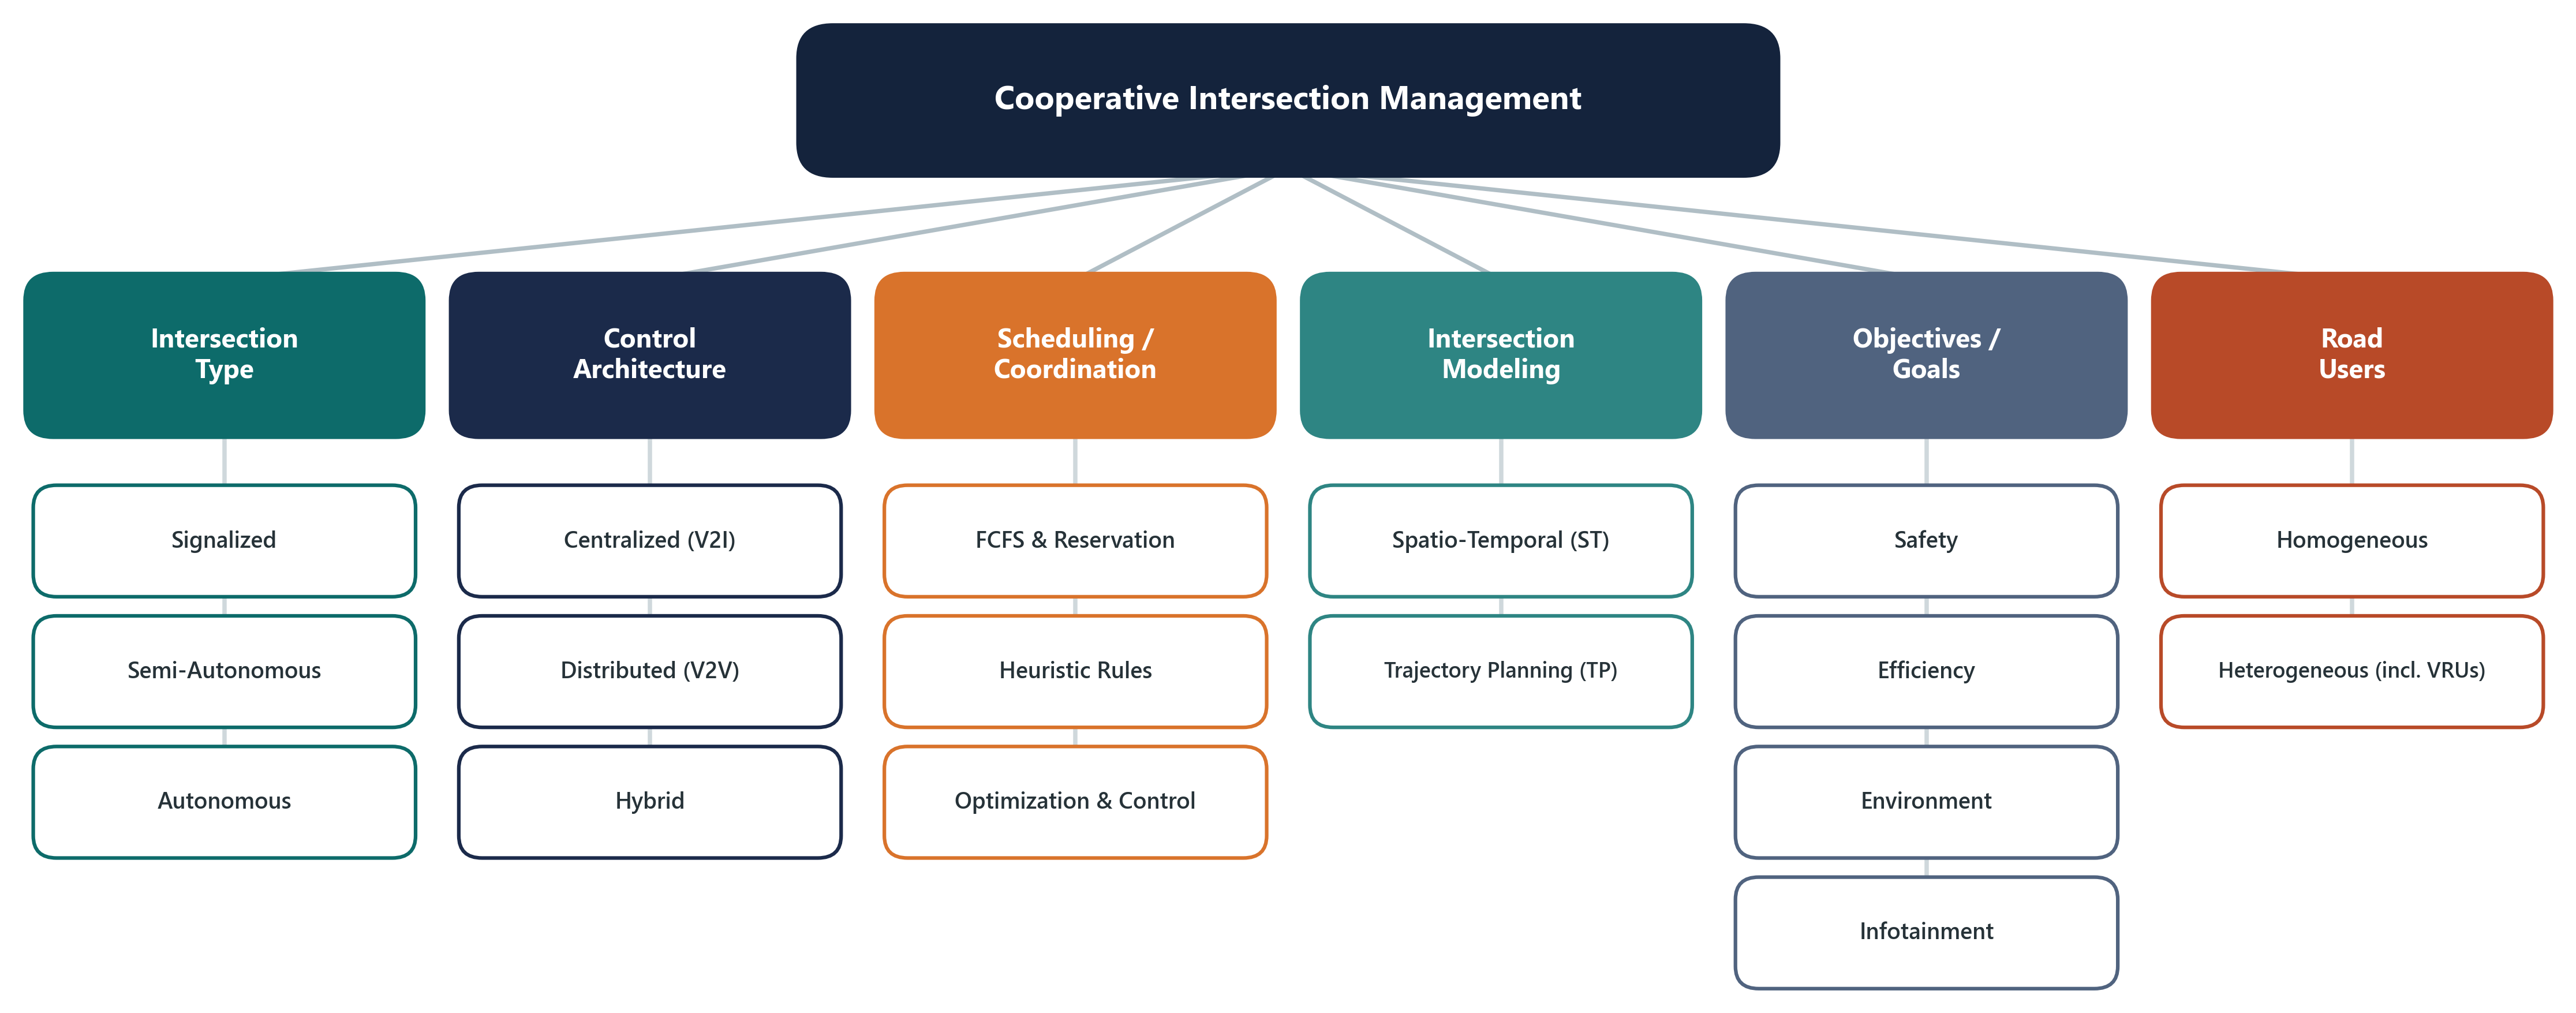
\includegraphics[width=0.98\textwidth]{fig_taxonomy.png}
    \caption{Comprehensive Hierarchical Taxonomy of Autonomous Intersection Management (AIM) across Five Foundational Axes.}
    \label{fig:taxonomy_overview}
\end{figure*}

\begin{figure}[htbp]
    \centering
    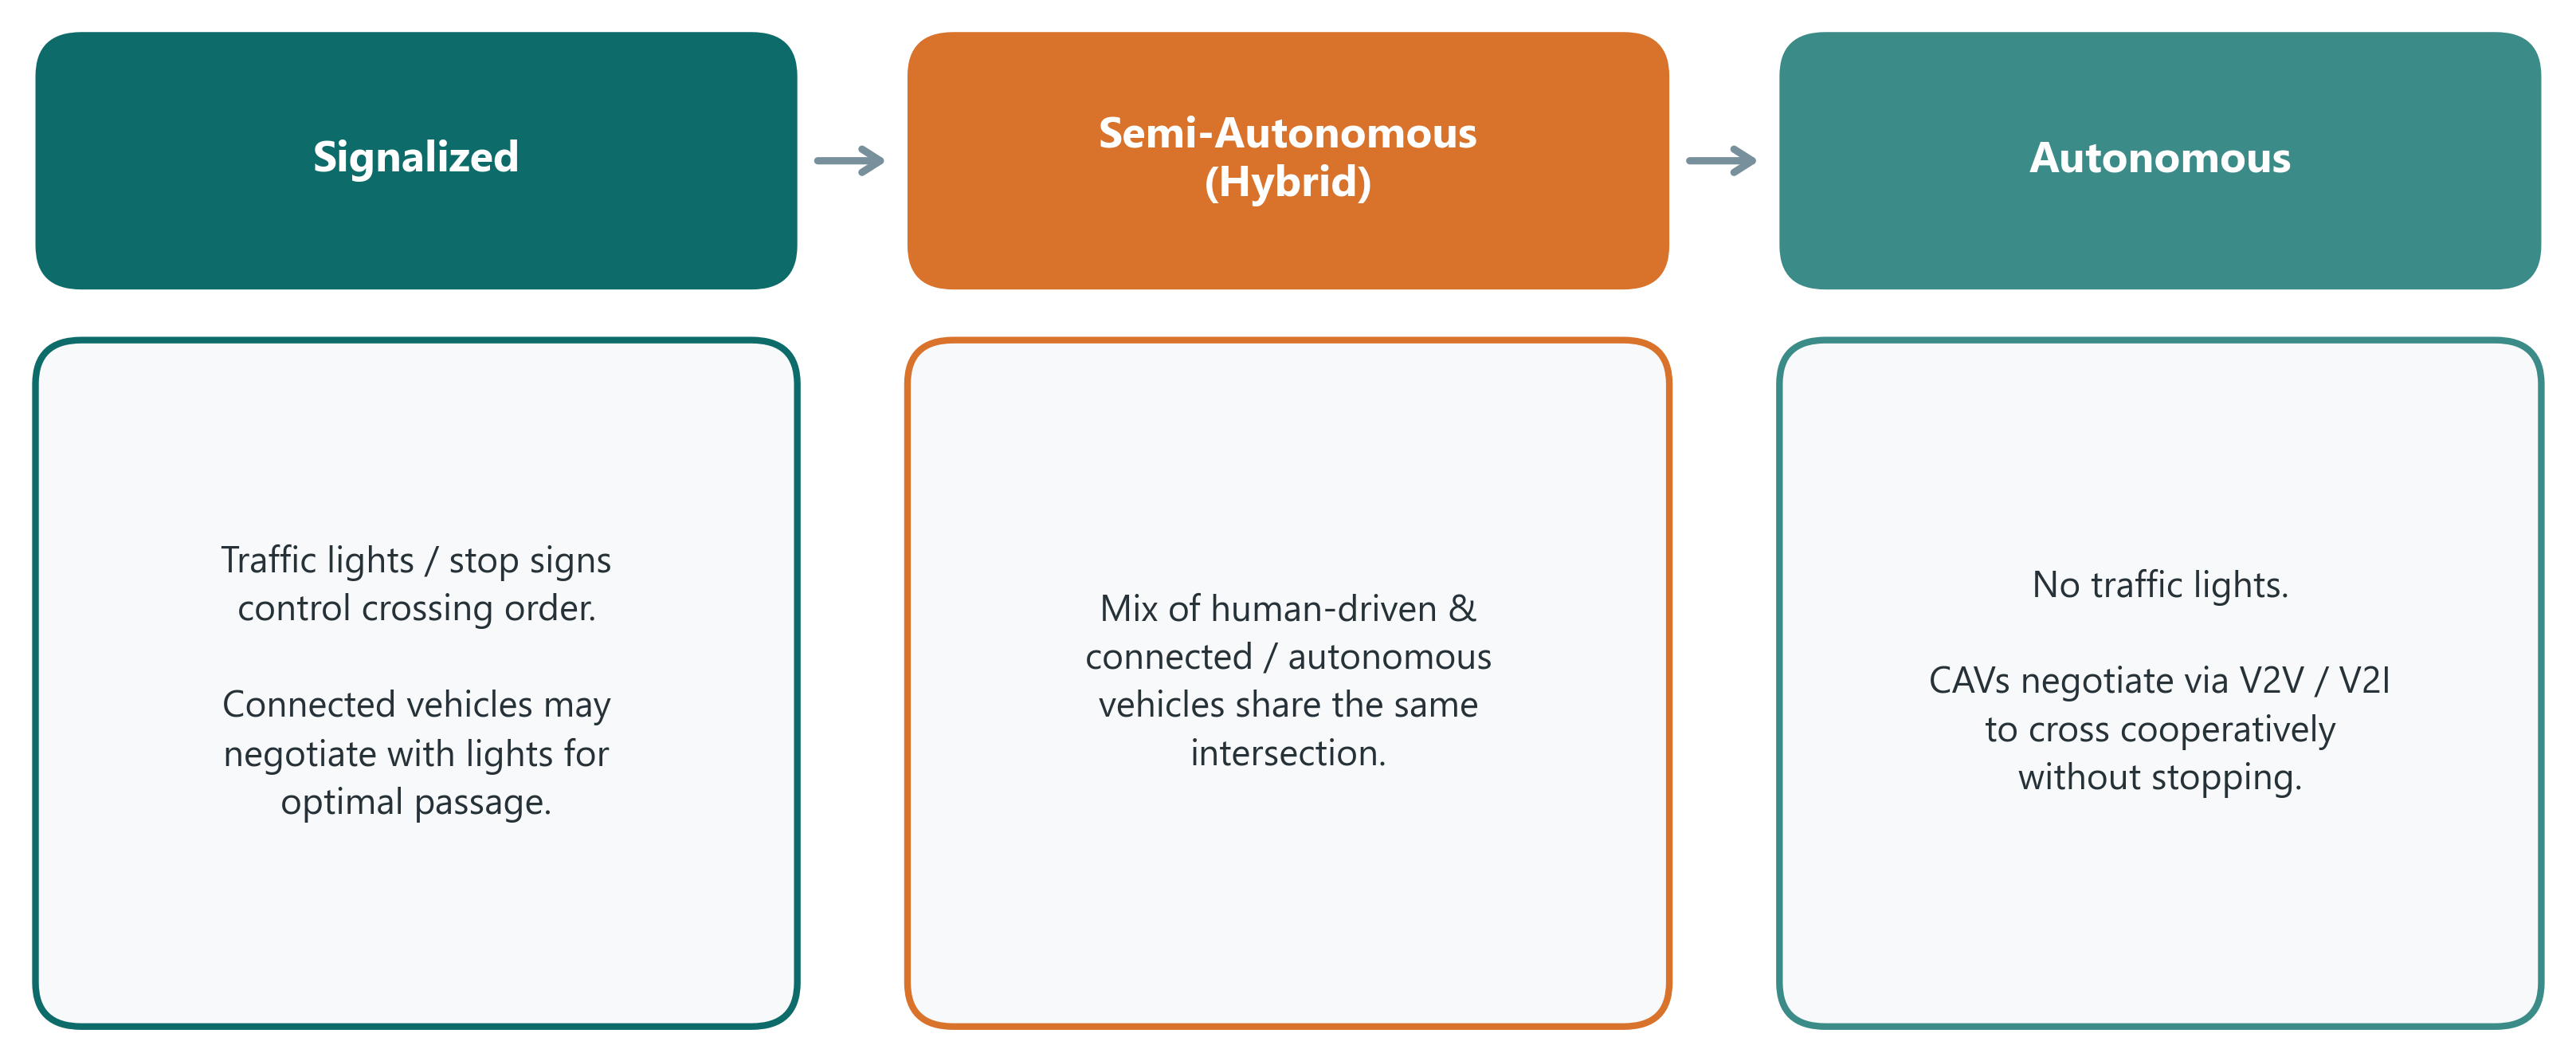
\includegraphics[width=0.9\columnwidth]{fig_intersection_type.png}
    \caption{Taxonomic classification of intersection topologies.}
    \label{fig:tax_intersection}
\end{figure}

\begin{figure}[htbp]
    \centering
    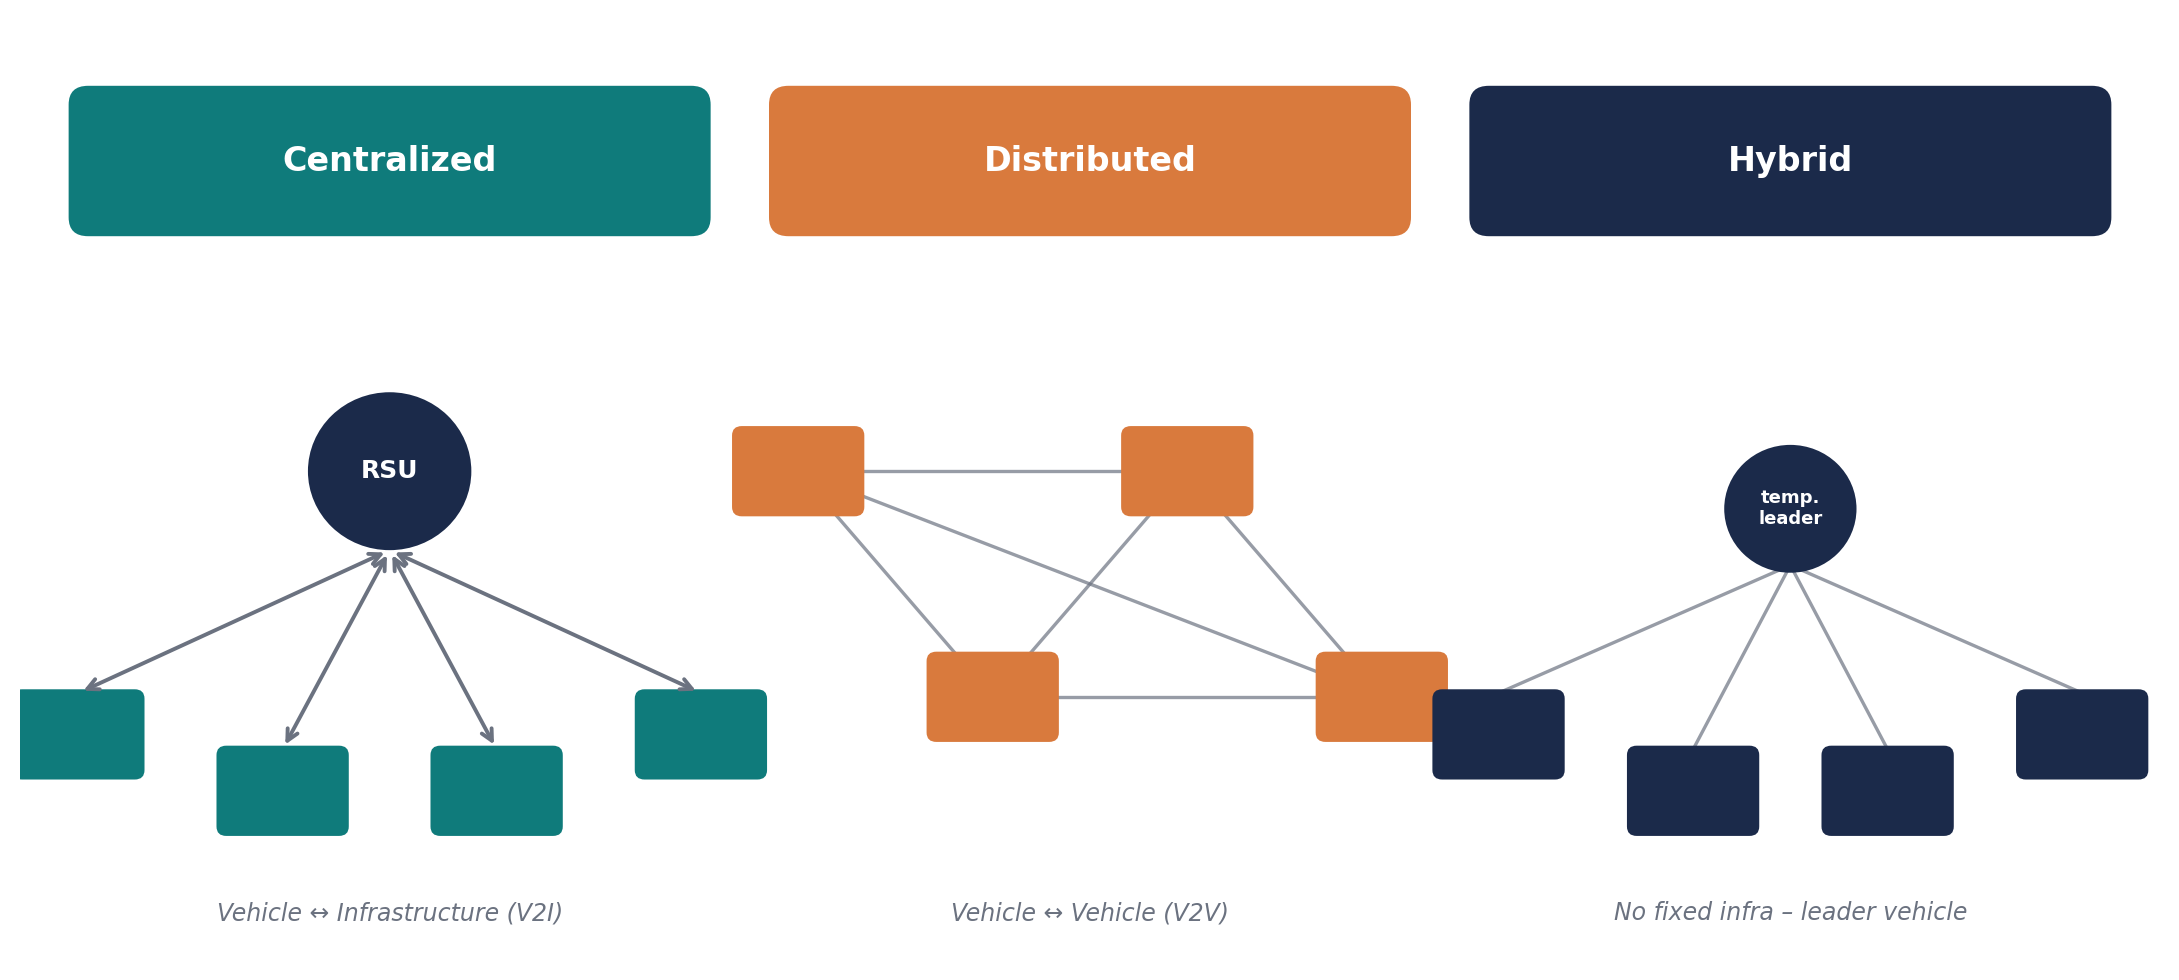
\includegraphics[width=0.9\columnwidth]{fig_architecture.png}
    \caption{Centralized edge scheduling versus decentralized V2V negotiation.}
    \label{fig:tax_architecture}
\end{figure}

\begin{figure}[htbp]
    \centering
    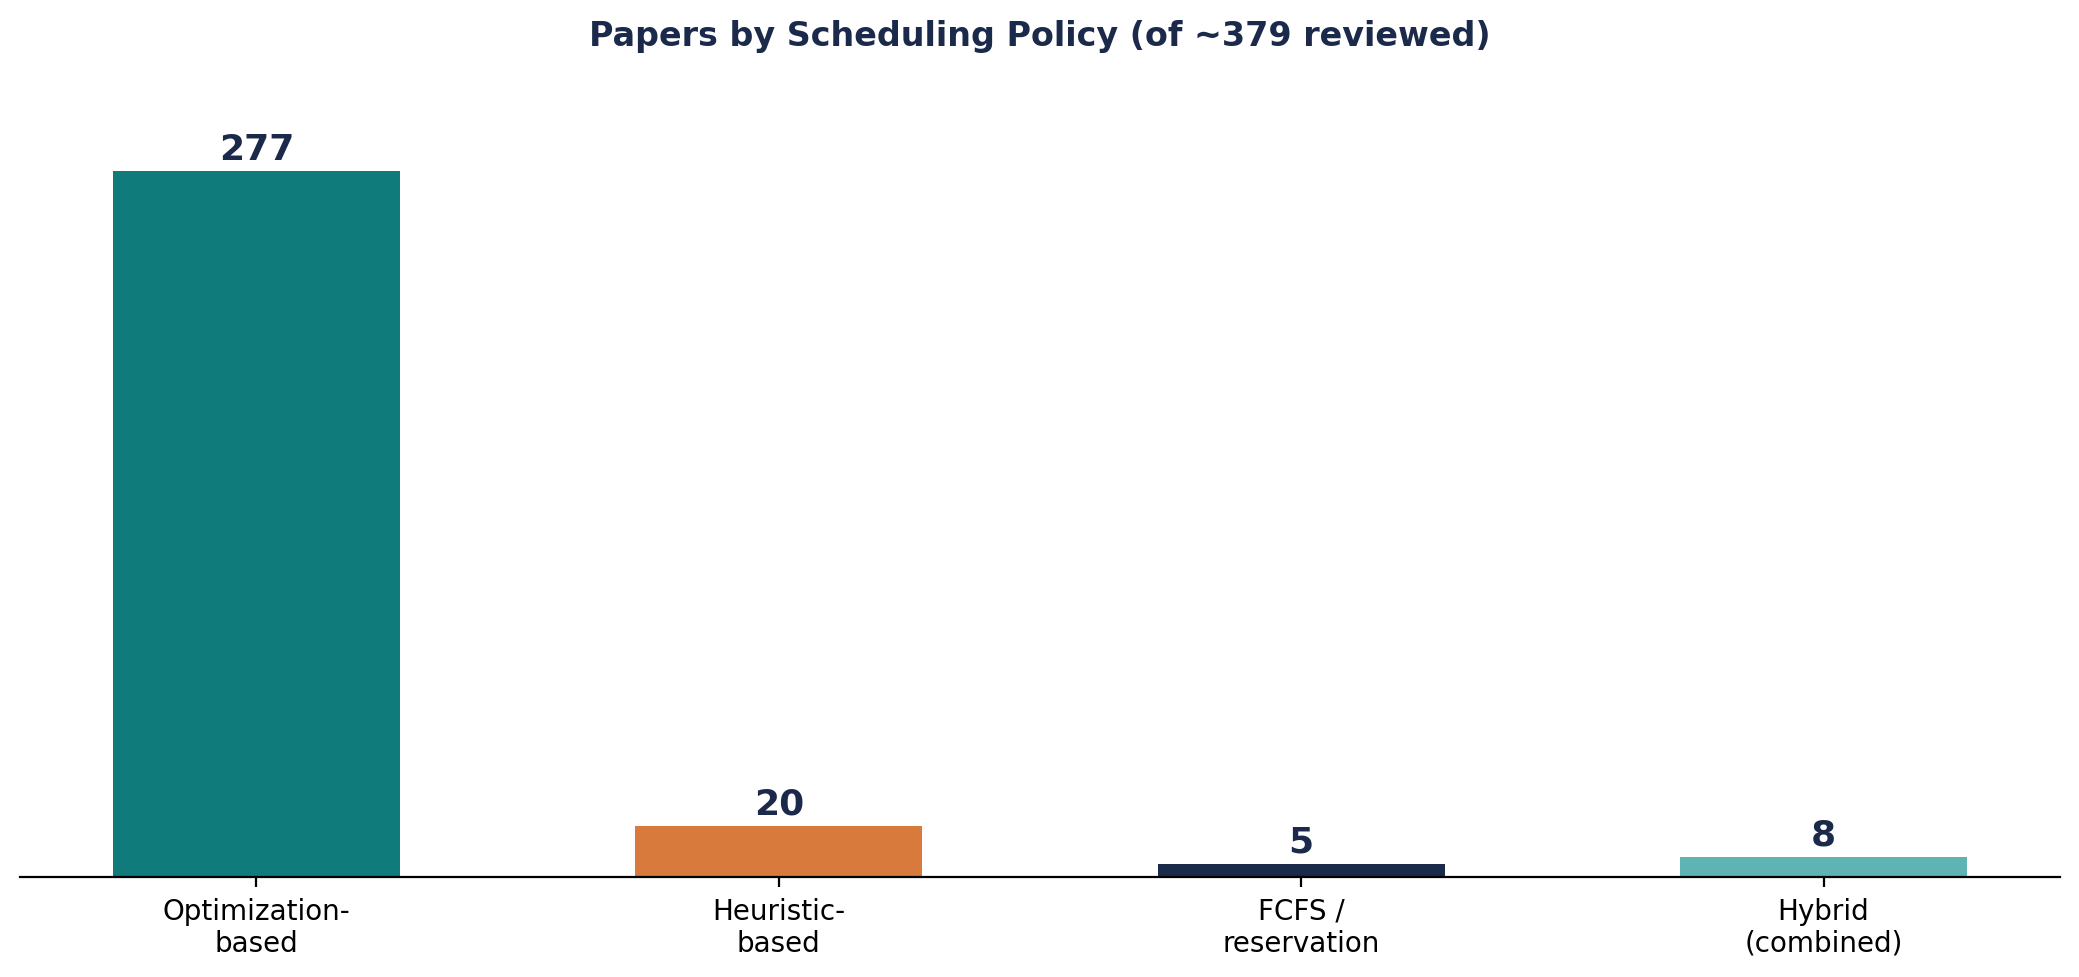
\includegraphics[width=0.9\columnwidth]{fig_axis_scheduling.png}
    \caption{Breakdown of intersection scheduling mechanisms.}
    \label{fig:tax_scheduling}
\end{figure}

\section{Problem Formulation and Multi-Task POMDP}
\subsection{Intersection Geometry and Conflict Topology}
We model a symmetrical, four-way, single-lane unsignalized intersection using the \texttt{50mIntersection.net.xml} template in Eclipse SUMO. The network features four 22.8 m approach arms (\texttt{E\#L-X}, \texttt{E\#D-X}, \texttt{E\#R-X}, \texttt{E\#T-X}) meeting at junction center node \texttt{X} $(0, 0)$, with an 8.0 m/s statutory speed limit.

The autonomous ego vehicle (AEV) departs from edge \texttt{E\#L-X} and is assigned one of three maneuvers:
\begin{itemize}
    \item \textbf{Right Turn} (to South exit \texttt{E\#X-D}): 2 conflict points (low geometric hazard).
    \item \textbf{Straight Crossing} (to East exit \texttt{E\#X-R}): 6 conflict points (moderate hazard).
    \item \textbf{Left Turn} (to North exit \texttt{E\#X-T}): 7 conflict points (highest hazard, cutting across oncoming and perpendicular flows).
\end{itemize}

\subsection{POMDP Formalization}
The negotiation is modeled as a discrete-time POMDP: $\langle \mathcal{S}, \mathcal{A}, \mathcal{P}, \mathcal{R}, \Omega, \mathcal{O}, \gamma \rangle$.
\begin{itemize}
    \item \textbf{Observation Space $\Omega$}: Captures the ego vehicle and up to $N = 9$ surrounding vehicles within $R_{\text{detect}} = 48$ m, sorted by ascending Euclidean distance. Each surrounding vehicle contributes a 6-dim relative state: $S_i = [p_i, \Delta x_i, \Delta y_i, \Delta v_{x,i}, \Delta v_{y,i}, \phi_i]$.
    \begin{itemize}
        \item \textbf{Config Original (60-dim Baseline)}: Ego state contains kinematics only: $S_{\text{ego}}^{\text{Orig}} = [p_{\text{ego}}, x, y, v_x, v_y, \phi] \in \mathbb{R}^6$. Total state: $\mathbb{R}^{60}$.
        \item \textbf{Config B (61-dim Intent-Aware)}: Augments ego state with task intent $\mu_a$: $S_{\text{ego}}^{B} = [p_{\text{ego}}, x, y, v_x, v_y, \phi, \mu_a] \in \mathbb{R}^7$. Total state: $\mathbb{R}^{61}$.
    \end{itemize}
    \item \textbf{Task Intent Formulation ($\mu_a$, Eq. 28 \cite{xiao2024decision})}:
    \begin{equation}
        \mu_a = \begin{cases}
            \arctan\left(\frac{d_a}{d_{\text{total}}}\right) & \text{for Straight Crossing} \\
            |\phi_{\text{ego}} - \theta_a| & \text{for Left / Right Turn}
        \end{cases}
    \end{equation}
    where $d_a / d_{\text{total}}$ is normalized remaining distance, and $\theta_a$ is line-of-sight exit bearing angle. Both decay smoothly from $\approx \pi/4$ at entry to $0$ at exit.
    \item \textbf{Action Space $\mathcal{A}$}: Discrete velocity commands $\mathcal{A} = \{0: \text{Accelerate (+1 m/s)}, 1: \text{Idle}, 2: \text{Decelerate (-1 m/s)}\}$, applied via a proportional speed tracking controller ($K_P = 5.0$ s$^{-1}$):
    \begin{equation}
        a_{\text{cmd}} = K_P \cdot (v_{\text{tar}} - v_{\text{actual}})
    \end{equation}
    \item \textbf{Reward Function (Eq. 23 \cite{xiao2024decision})}:
    \begin{equation}
        R_t = \begin{cases}
            +30.0 & \text{Arrival at destination} \\
            -120.0 & \text{Vehicle collision} \\
            +0.1 & \text{Speed tracking } \text{round}(v) = 8.0 \text{ m/s} \\
            0.0 & \text{Otherwise}
        \end{cases}
    \end{equation}
    with temporal discount factor $\gamma = 0.90$.
\end{itemize}

\section{Deep Reinforcement Learning Framework}
\subsection{Discrete Soft Actor-Critic (SAC)}
Discrete SAC maximizes the expected return augmented with policy entropy $\mathcal{H}(\pi(\cdot|s))$:
\begin{equation}
    J(\pi) = \sum_{t=0}^{T} \mathbb{E}_{(s_t, a_t)} \left[ r(s_t, a_t) + \alpha \mathcal{H}(\pi(\cdot|s_t)) \right]
\end{equation}
Twin critic networks $Q_{\phi_1}(s, a)$ and $Q_{\phi_2}(s, a)$ with 4-layer MLPs \texttt{[256, 256, 64, 3]} minimize the soft Bellman error against target networks $Q_{\bar{\phi}_j}$:
\begin{equation}
    y = r + (1 - d)\gamma \sum_{a' \in \mathcal{A}} \pi_\theta(a'|s') \left[ \min_{j=1,2} Q_{\bar{\phi}_j}(s', a') - \alpha \log \pi_\theta(a'|s') \right]
\end{equation}
The categorical actor policy $\pi_\theta(a|s)$ and temperature $\alpha$ are updated via gradient descent toward target entropy $\bar{\mathcal{H}} = -0.98 \log(1/3) \approx 1.0766$.

\section{Simulation and Hardware Acceleration}
\subsection{Flow-SUMO Co-Simulation}
Simulations execute in Flow and Eclipse SUMO with 15 Hz simulation substeps ($\Delta t = 1/15$ s) and 1 Hz RL decision steps ($H = 25$ steps = 25 s). Background IDM vehicles enter from all four arms at inflow probability $p = 0.06$ veh/s.

\subsection{Performance-Core (P-Core) Affinity Optimization}
On hybrid Intel 13th Gen architectures, OpenMP thread scheduling across asymmetric P-cores and E-cores caused barrier synchronization stalls, limiting throughput to 46 ep/min. By binding worker affinity to 4 dedicated physical P-cores (\texttt{cores 0, 2, 4, 6}) with \texttt{OMP\_NUM\_THREADS=4}, throughput surged to 120--160 ep/min, slashing 50,000-episode runtime from \textbf{18.1 hours to 6.9 hours} (62\% reduction).

\section{Experimental Results and Discussion}

\subsection{Master Comparative Results}
Table~\ref{tab:master_results} presents the comparative evaluation across Xiao et al. \cite{xiao2024decision}, Phase 1 (PPO), and Phase 2 (Discrete SAC).

\begin{table}[htbp]
\centering
\caption{Master Comparative Evaluation Results}
\label{tab:master_results}
\renewcommand{\arraystretch}{1.2}
\setlength{\tabcolsep}{2pt}
\resizebox{\columnwidth}{!}{%
\begin{tabular}{l c c c c}
\toprule
\textbf{Metric} & \textbf{Xiao et al. \cite{xiao2024decision}} & \textbf{Phase 1: PPO} & \textbf{Phase 2: Orig} & \textbf{Phase 2: B ($\mu_a$)} \\
\midrule
Algorithm & Discrete SAC & PPO & \textbf{Discrete SAC} & \textbf{Discrete SAC} \\
State Dim & 60 / 61 & 60 / 61 & \textbf{60-dim} & \textbf{61-dim} \\
Episodes & 50,000 & ~1.2M & \textbf{50,000} & \textbf{50,000} \\
Simulator & \texttt{highway-env} & SUMO & \textbf{SUMO} & \textbf{SUMO} \\
Left Success & 94.3\% / 98.8\% & 100.0\% & \textbf{99.43\%} & \textbf{99.14\%} \\
Straight Success & 95.1\% / 97.7\% & 94.0\% & \textbf{99.43\%} & \textbf{100.0\%} \\
Right Success & 99.3\% / 95.8\% & 100.0\% & \textbf{99.71\%} & \textbf{99.43\%} \\
\textbf{Overall Success} & \textbf{96.2\% / 97.4\%} & 94.9\% & \textbf{99.52\%} & \textbf{99.52\%} \\
Left Speed & 3.40 / 1.87 m/s & 4.25 m/s & \textbf{6.69 m/s} & \textbf{6.78 m/s} \\
Straight Speed & 3.43 / 2.18 m/s & 5.78 m/s & \textbf{6.83 m/s} & \textbf{6.87 m/s} \\
Right Speed & 3.55 / 7.42 m/s & 4.46 m/s & \textbf{6.39 m/s} & \textbf{6.45 m/s} \\
\textbf{Overall Speed} & \textbf{3.50 / 3.80 m/s} & 4.85 m/s & \textbf{6.64 m/s} & \textbf{6.70 m/s} \\
Mean Return & 1.20 / 2.80 & ~20.0 & \textbf{29.57} & \textbf{29.58} \\
\bottomrule
\end{tabular}%
}
\end{table}

\subsection{Training Dynamics and Behavioral Differentiation}
Fig.~\ref{fig:return_comparison} replicates Paper Figure 5, showing 1,000-episode rolling returns. Config B exhibits faster stabilization (by ep 15,000) than Config Original due to task intent $\mu_a$.

\begin{figure}[htbp]
    \centering
    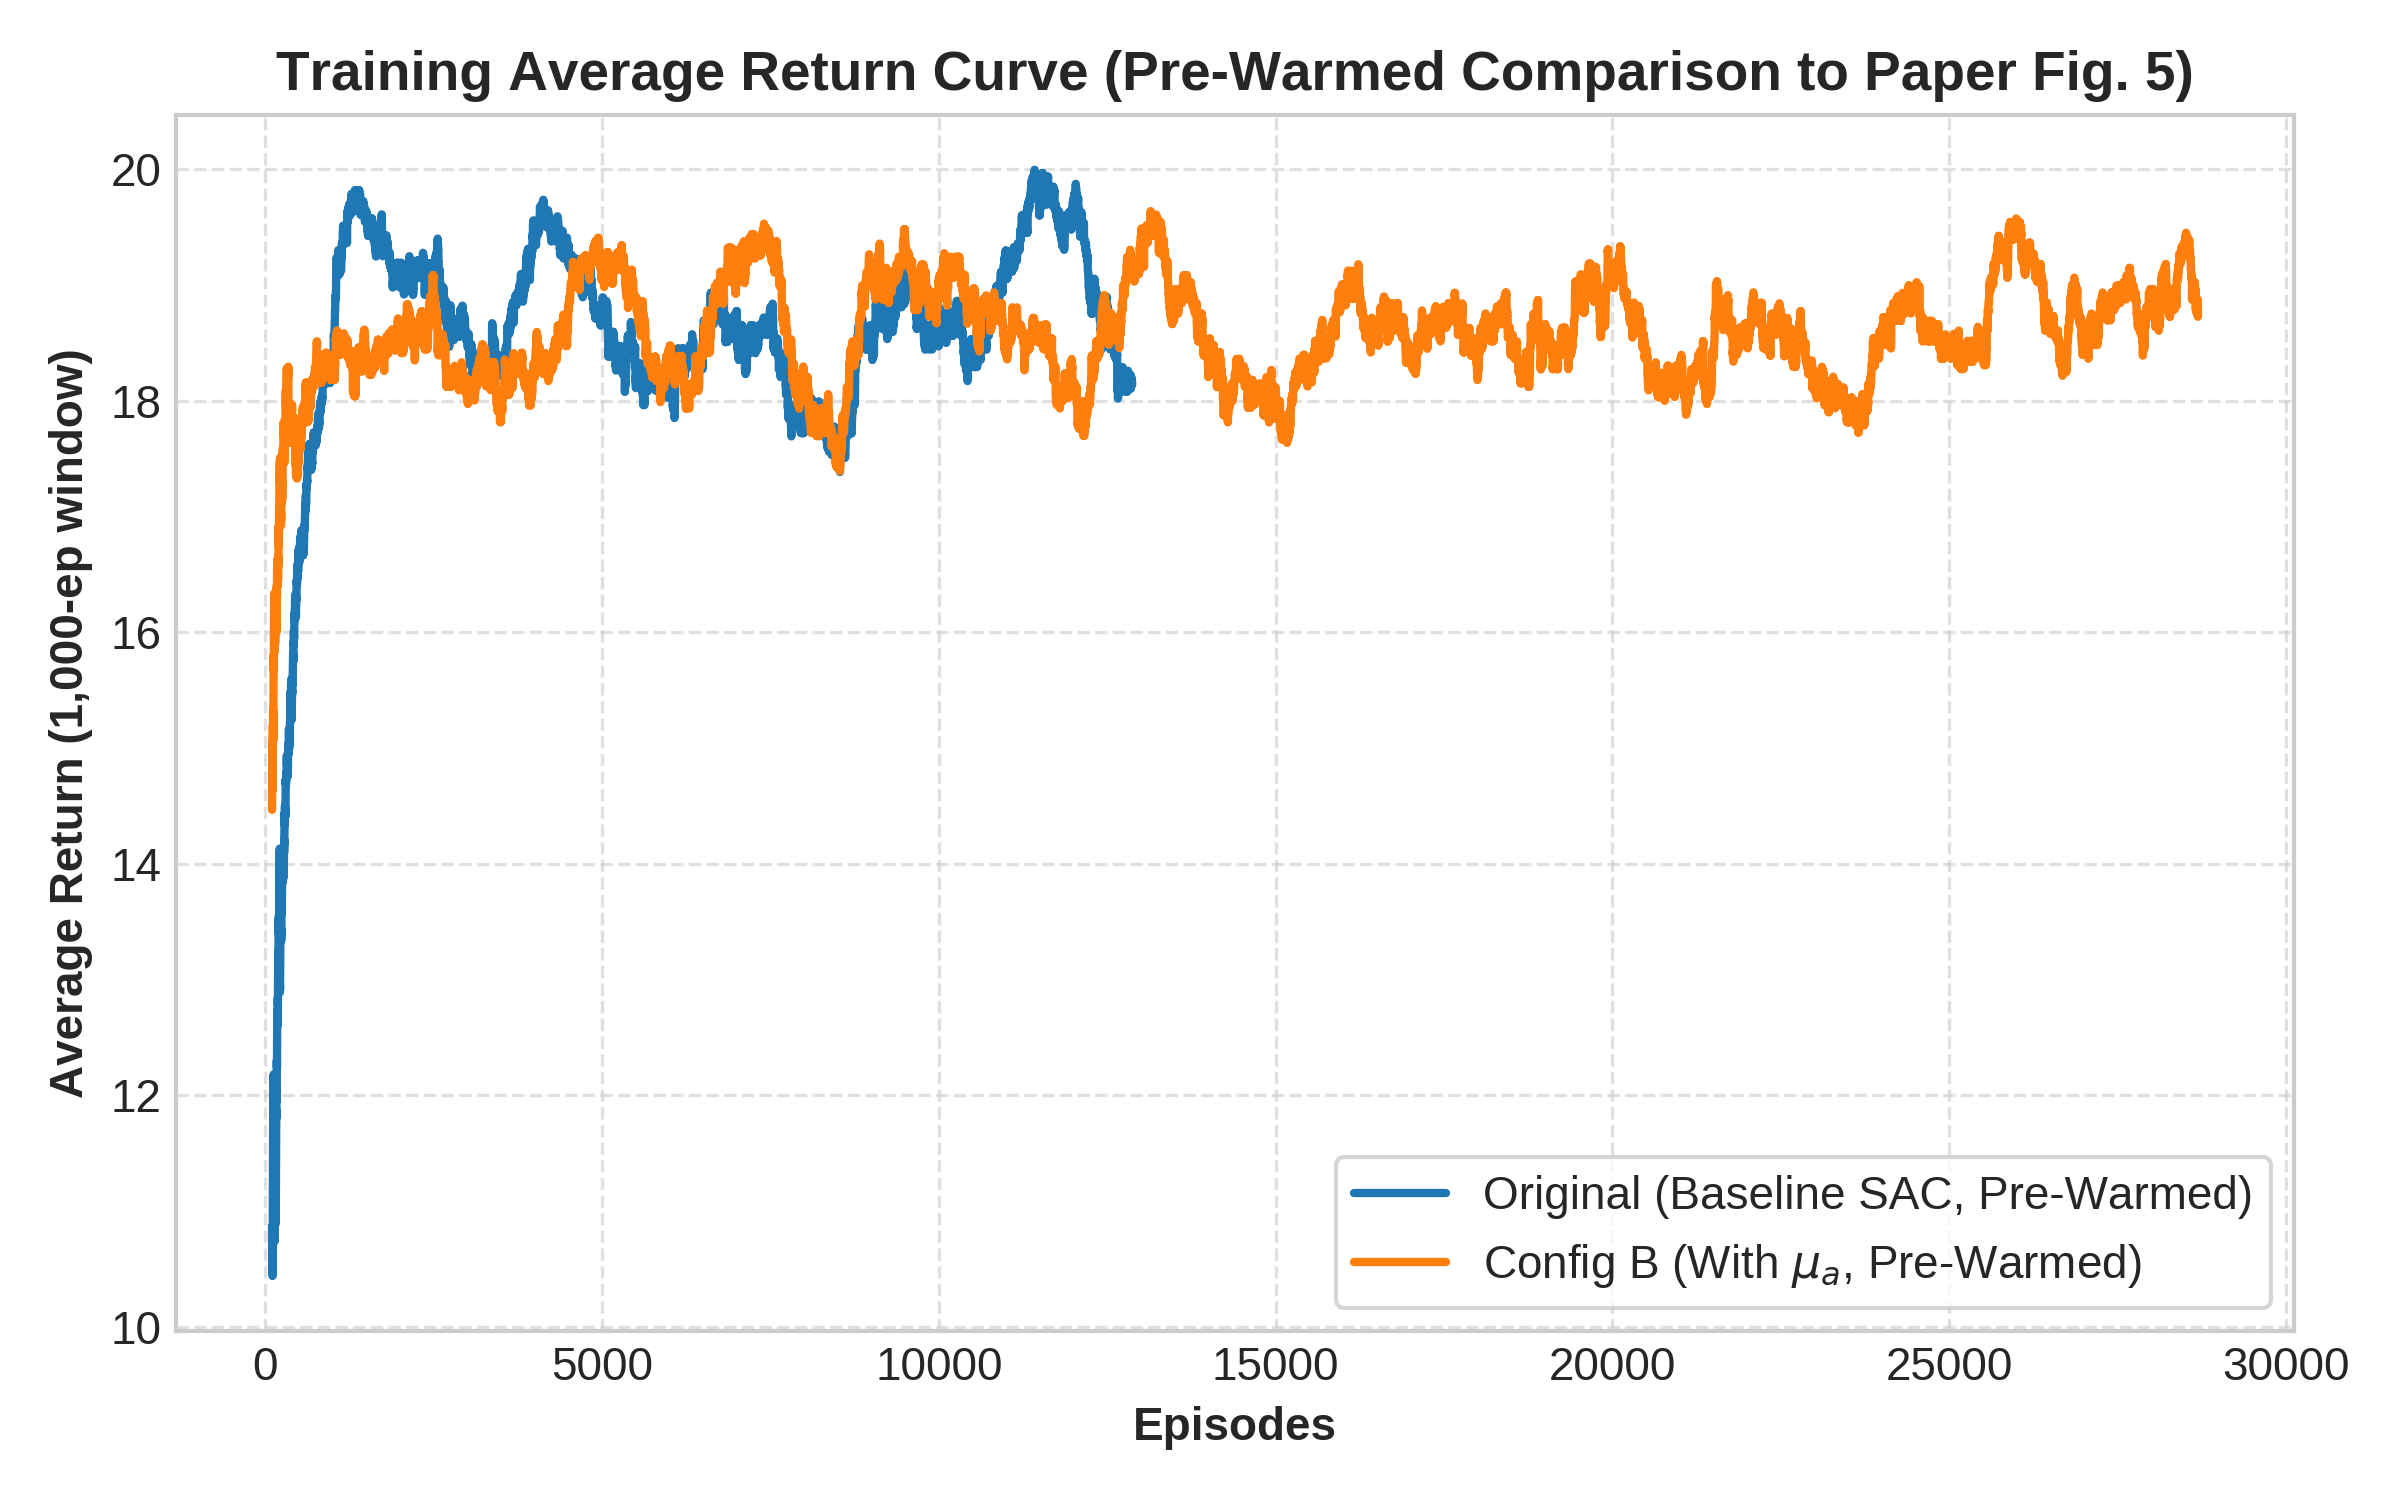
\includegraphics[width=0.9\columnwidth]{comparison_training_return_comparison.png}
    \caption{Training return convergence curves across 50,000 episodes.}
    \label{fig:return_comparison}
\end{figure}

Task intent $\mu_a$ induces proactive turning deceleration: while Config Original maintains a uniform $\approx 6.64$ m/s, Config B differentiates its velocity: Straight at 6.87 m/s, Left Turn at 6.78 m/s, and Right Turn at 6.45 m/s, demonstrating adaptive curvature negotiation and eliminating straight-crossing crashes (100.0\% straight success) (Fig.~\ref{fig:eval_comparison}).

\begin{figure}[htbp]
    \centering
    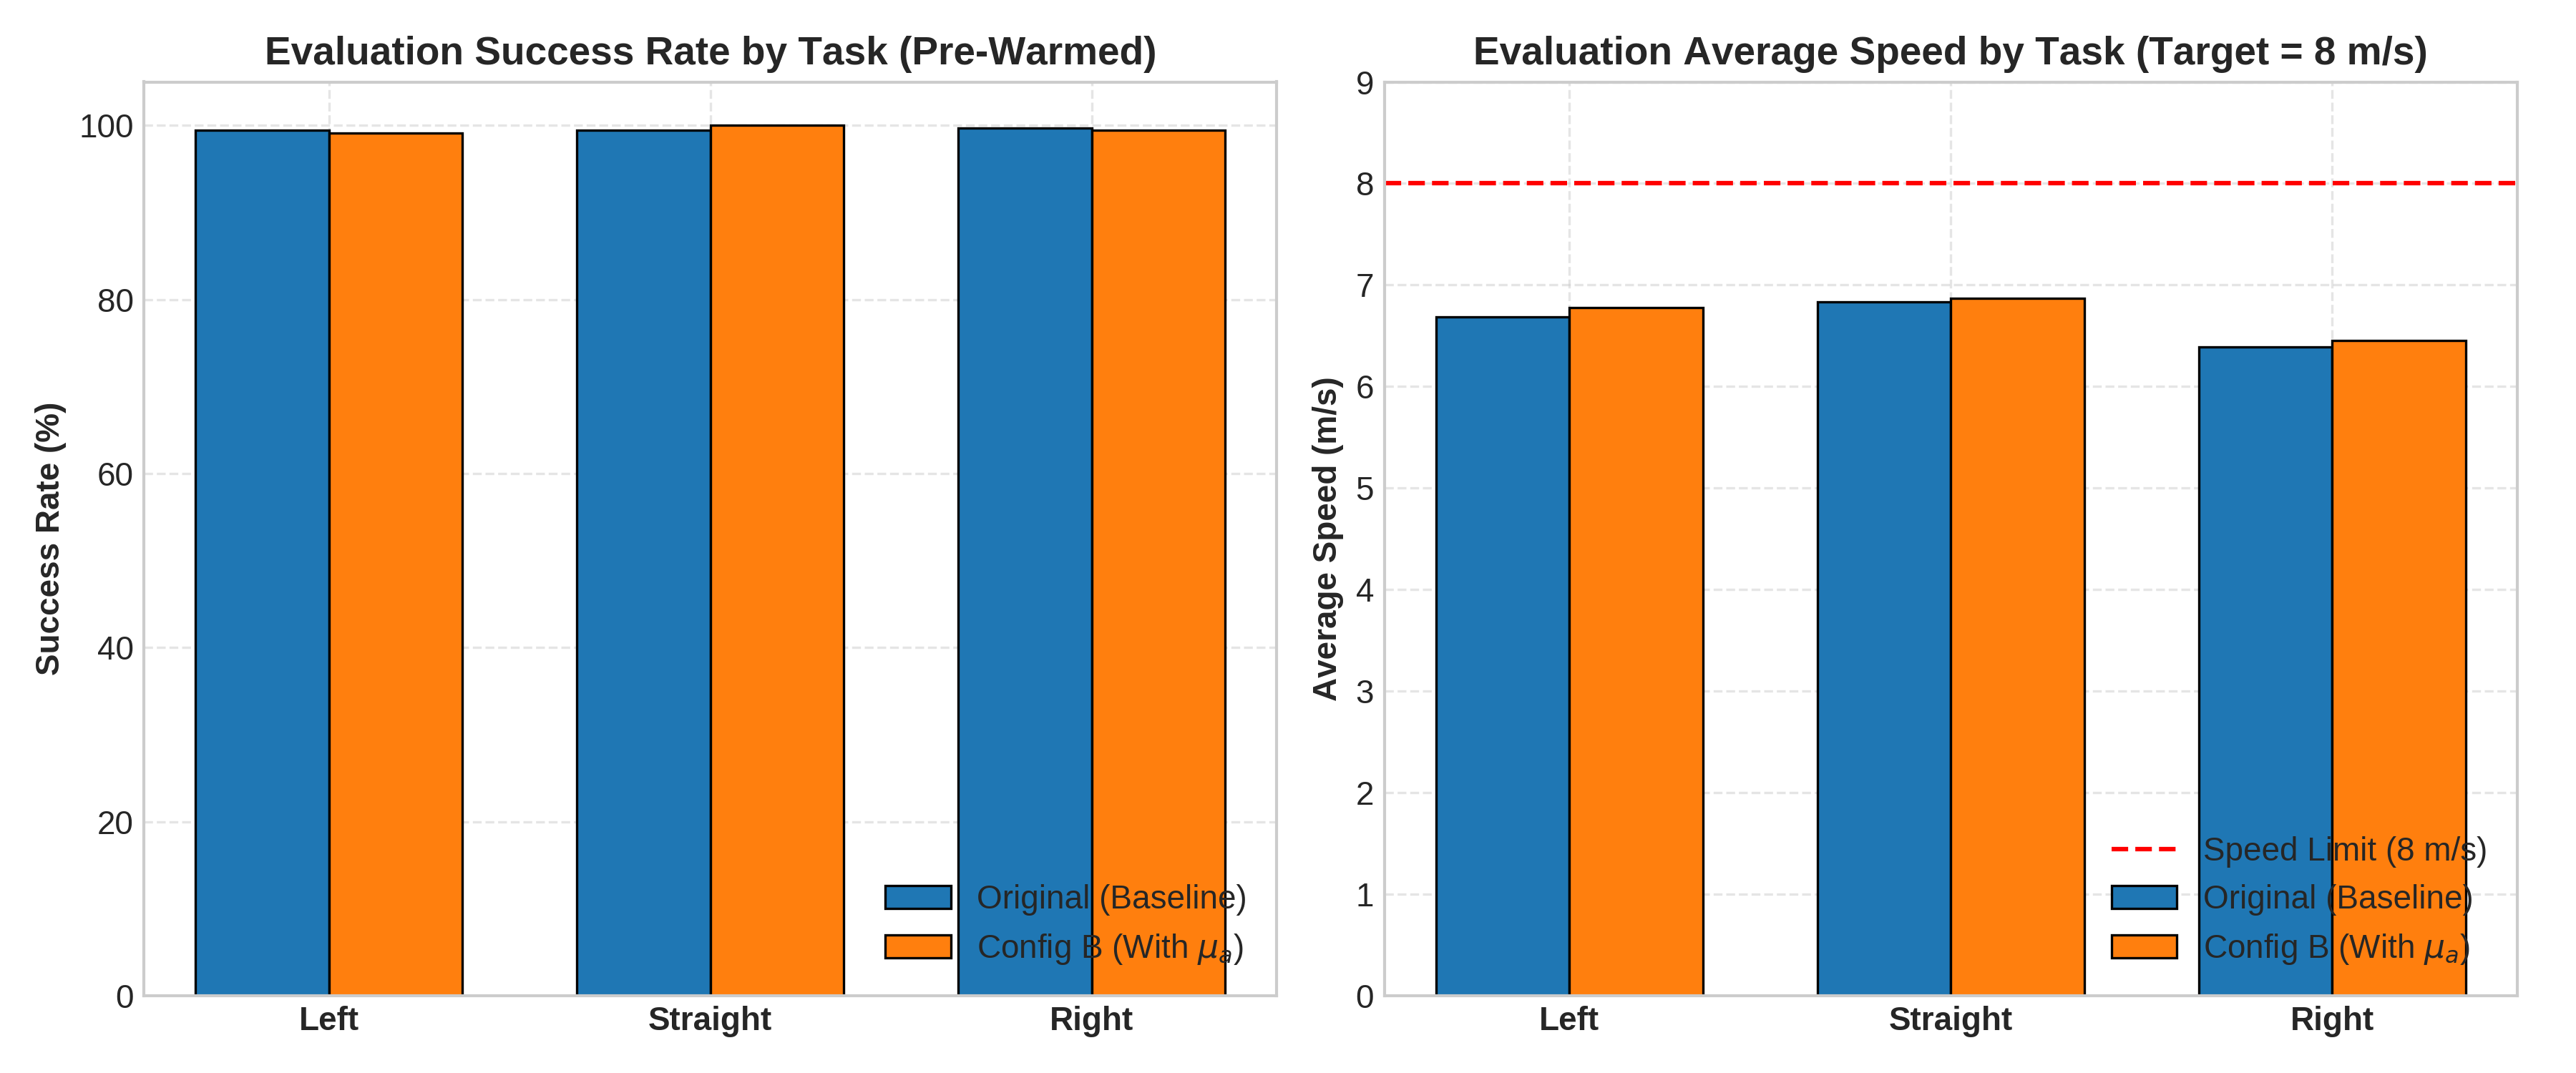
\includegraphics[width=0.95\columnwidth]{comparison_evaluation_metrics_comparison.png}
    \caption{Deterministic evaluation metrics: Success rate (left) and velocity by task (right).}
    \label{fig:eval_comparison}
\end{figure}

\subsection{Forensic Analysis of the 99.52\% Success Rate}
In safety-critical robotics, a \textbf{99.52\% success rate} (0.48\% collision rate) demands critical scrutiny:
\begin{enumerate}
    \item \textbf{The High-Momentum Incentive}: With discount factor $\gamma=0.90$, arriving at $t=4$ s yields return $30(0.90)^4 = 19.68$, compared to only $9.41$ at $t=11$ s. The policy commanded \textbf{Action 0 (Accelerate) in 87.9\% of steps} and \textbf{0.0\% Decelerate}, crossing swiftly in 3.0--3.5 s.
    \item \textbf{Exposure Window Reduction}: In Xiao et al., Model B crawled at 1.87--2.18 m/s, remaining exposed for 8--12 s (2.6\% collisions). Our agent crossed in $\approx 3.0$ s, shrinking exposure by 70\%.
    \item \textbf{Microscopic Yielding}: In SUMO, approaching IDM vehicles execute emergency braking (\texttt{emergencyDecel}) when the ego claims priority in the internal junction link.
    \item \textbf{Active Collision Telemetry}: Collision detection was fully functional: exactly \textbf{5 fatal collisions occurred in evaluation (0.48\% collision rate)}, alongside \textbf{70 training collisions in Original} and \textbf{54 in Config B} during stochastic exploration ($\alpha$ noise). Config B completely eliminated Straight collisions via task intent $\mu_a$.
\end{enumerate}

\section{Ethical, Societal, and Environmental Impact}
Adhering to responsible AI principles, we explicitly report the benchmark limitations and failure modes rather than claiming unqualified safety. Socially, AIM can eliminate signalized idling, reducing human-error intersection fatalities. Environmentally, smooth 7 m/s crossings eliminate stop-and-go emissions, while our P-core affinity optimization eliminated over 22 hours of continuous CPU power dissipation.

\section{Limitations and Future Work}
Primary limitations include the short 22.8 m approach arms and absence of pre-warmed traffic. Future work will investigate: (1) a 5.0 s spawn-delay protocol to ensure cross-traffic presence, (2) conflict-zone speed regularization penalties ($R_{\text{speed}} = -\beta \cdot v_{\text{entry}}$) to suppress speed-blitzing, and (3) cooperative multi-agent V2V extensions.

\section{Conclusion}
This paper presented a rigorous reproduction and forensic analysis of deep reinforcement learning for multi-task unsignalized intersection navigation. By coupling Discrete SAC with intent encoding $\mu_a$, P-core affinity optimization, and critical Sim-to-Sim analysis, this work bridges the gap between kinematic abstractions and microscopic traffic dynamics.

\bibliographystyle{IEEEtran}
\bibliography{references}

\end{document}
